\section{Introduction}
\label{sec:intro}

Grammar rules apply not to individual words (e.g. dog, eat) but to
syntactic categories of words (e.g. noun, verb).  Thus constructing
syntactic categories (also known as lexical or part-of-speech
categories) is one of the fundamental problems in language
acquisition.

Syntactic categories represent groups of words that can be substituted
for one another without altering the grammaticality of a sentence.
Linguists identify syntactic categories based on semantic, syntactic,
and morphological properties of words.  There is also evidence that
children use prosodic and phonological features to bootstrap syntactic
category acquisition \cite{ambridge2011child}.  However there is as
yet no satisfactory computational model that can match human
performance.  Thus identifying the best set of features and best
learning algorithms for syntactic category acquisition is still an
open problem.

\begin{figure}[b] 
  \centering
  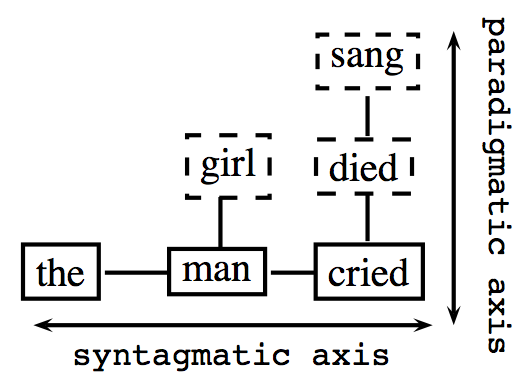
\includegraphics[height=50mm,width=50mm]{paradigmatic.png}
  \caption{Syntagmatic vs. paradigmatic axes for words in a simple
    sentence \protect\cite{chandler2007semiotics}.}
  \label{fig:paradigmatic}
\end{figure}

Relationships between linguistic units can be classified into two
types: syntagmatic (concerning positioning), and paradigmatic
(concerning substitution).  Syntagmatic relations determine which
units can combine to create larger groups and paradigmatic relations
determine which units can be substituted for one another.
Figure~\ref{fig:paradigmatic} illustrates the paradigmatic vs
syntagmatic axes for words in a simple sentence and their possible
substitutes.  

In this study, we represent the paradigmatic axis directly by building
{\em substitute vectors} for each word position in the text.  The
dimensions of a substitute vector represent words in the vocabulary,
and the magnitudes represent the probability of occurrence in the given
position.  Note that the substitute vector for a word position (e.g.
the second word in Fig.~\ref{fig:paradigmatic}) is a function of the
context only (i.e. ``the \_\_\_ cried''), and does not depend on the
word that does actually appear there (i.e. ``man'').  Thus substitute
vectors represent {\em individual word contexts}, not word types.  We
refer to the use of features based on substitute vectors as 
{\em paradigmatic representations of word context}.

Our preliminary experiments indicated that using context information
alone without the identity or the features of the target word
(e.g. using dimensionality reduction and clustering on substitute
vectors) has limited success and modeling the co-occurrence of word
and context types is essential for inducing syntactic categories.  In
the models presented in this paper, we combine paradigmatic
representations of word context with features of co-occurring words
within the co-occurrence data embedding (CODE) framework
\cite{globerson2007euclidean,maron2010sphere}.  The resulting
embeddings for word types are split into 45 clusters using k-means and
the clusters are compared to the 45 gold tags in the 1M word Penn
Treebank Wall Street Journal corpus \cite{treebank3}.  We obtain
many-to-one accuracies up to .7680 using only distributional
information (the identity of the word and a representation of its
context) and .8023 using morphological and orthographic features of
words improving the state-of-the-art in unsupervised part-of-speech
tagging performance.

% example substitute vectors (both syntactic and semantic)
The high probability substitutes reflect both semantic and syntactic
properties of the context as seen in the example below (the numbers in
parentheses give substitute probabilities):

\begin{quote}
\noindent {\em ``Pierre Vinken, 61 years old, will join the board as a nonexecutive director Nov.~29.''}\\
\noindent {\bf the:} its (.9011), the (.0981), a (.0006), $\ldots$\\
{\bf board:} board (.4288), company (.2584), firm (.2024), bank (.0731), $\ldots$
\end{quote}

Top substitutes for the word ``the'' consist of words that can act as
determiners.  Top substitutes for ``board'' are not only nouns, but
specifically nouns compatible with the semantic context.

This example illustrates two concerns inherent in all distributional
methods: (i) words that are generally substitutable like ``the'' and
``its'' are placed in separate categories ({\sc dt} and {\sc prp\$})
by the gold standard, (ii) words that are generally not substitutable
like ``do'' and ``put'' are placed in the same category ({\sc vb}).
Freudenthal et al. \shortcite{freudenthal2005resolution} point out
that categories with unsubstitutable words fail the standard
linguistic definition of a syntactic category and children do not seem
to make errors of substituting such words in utterances
(e.g. {\em``What do you want?''}  vs. {\em *``What put you want?''}).
Whether gold standard part-of-speech tags or distributional categories
are better suited to applications like parsing or machine translation
can be best decided using extrinsic evaluation.  However in this study
we follow previous work and evaluate our results by comparing them to
gold standard part-of-speech tags.

Section~\ref{sec:related} gives a detailed review of related work.
Section~\ref{sec:subthr} describes the construction of the substitute
vectors.  Section~\ref{sec:subapp} analyzes the limits of solely using
substitute vectors on a sample data set.  Section~\ref{sec:code}
describes co-occurrence data embedding, the learning algorithm used in
our experiments.  Section~\ref{sec:exp} describes possible usage
scenerios of substitute vectors with S-Code on English and determines
the best setup.  Section~\ref{sec:multilang} applies the best setup to
different languages and compares with previous work.
Section~\ref{sec:discuss} gives a brief error analysis and
Section~\ref{sec:contrib} summarizes our contributions.  All the data
and the code to replicate the results given in this paper is available
from the authors' website at \mbox{\url{xxx.xxx.xxx}}.


%% Computational models of syntactic category acquisition rely mainly on
%% distributional analysis: Words that share the same distribution
%% (i.e. that occur in the same context) are grouped into the same
%% category.  The definition of ``the same context'' vary across studies.
%% Algorithms based on the Hidden Markov Model use class based n-grams to
%% specify context \cite{Brown:1992:CNG:176313.176316}, others use a
%% frame of neighboring words around the target word
%% \cite{Schutze:1995:DPT:976973.976994}.

%% Our hypothesis is that potential substitutes of a word are directly
%% indicative of its syntactic category and should be useful in acquiring
%% syntactic categories in general.  

%% Our main contribution in this study
%% is to introduce paradigmatic features, i.e. features based on
%% potential substitutes of the target word, to represent word context.

%% Both syntagmatic and paradigmatic relations of a word can be used to
%% represent its context.  In the syntagmatic case the context is
%% represented by a selection of neighboring words, in the paradigmatic
%% case it is represented by a set of possible substitutes.  In previous
%% studies of syntactic category learning the context representation has
%% been primarily syntagmatic, either implicit in the class based n-grams
%% of the standard Hidden Markov Model, or explicit in the construction
%% and clustering of left and right neighbors.

%% In this study we explore a paradigmatic representation of the context
%% of a word in syntactic category acquisition.  Specifically, the
%% context of a word is represented by a list of its possible substitutes
%% and their probabilities, which we call the {\em substitute vector}.
%% Note that the substitute vector is a function of the context only, not
%% the target word.  Thus in effect we are clustering contexts, not
%% words.  When word contexts are clustered based on their substitute
%% vectors they reveal a grouping that largely match the traditional part
%% of speech boundaries (\bestResult many-to-one score using a
%% 45-tag 24K word test corpus).
%% % standard HMM-EM gives 42\% on the same data.

%% Section~\ref{sec:related} gives a detailed review of related work.
%% The construction of the substitute vectors is described in
%% Section~\ref{sec:lm}.  To find out how to best make use of this new
%% paradigmatic representation, we explore different distance metrics
%% (Section~\ref{sec:dist}), dimensionality reduction methods
%% (Section~\ref{sec:dimreduce}), and clustering algorithms
%% (Section~\ref{sec:clustering}) for substitute vectors.  We note that
%% close to 95\% of the word occurrences in human labeled data are tagged
%% with their most frequent part of speech
%% \cite{Lee:2010:STU:1870658.1870741}, making one-tag-per-word a fairly
%% good first approximation.  Even ambicategory words generally have
%% fairly skewed part of speech distributions.
%% Section~\ref{sec:sparsity} looks at ways to increase the sparsity of
%% our solutions and demonstrates significant improvements using the
%% one-tag-per-word assumption and similarity metrics that introduce
%% sparsity.  Section~\ref{sec:discussion} discusses the results and
%% Section~\ref{sec:contrib} summarizes our contributions.

